\chapter{Lavoro ed energia}
\minitoc
\section{\index{lavoro}Lavoro definizione}
\begin{Def}[lavoro]
  Definiamo lavoro $L$ fatto dalla forza $\ve F$ sul punto $P$ di applicazione della forza lungo il percorso $\Gamma$ l'integrale su $\Gamma$ della forma differenziale $\delta L = \ve F\cdot\ud\ve s$:
  \begin{equation}
    L=\int_\Gamma\ve F\cdot\ud \ve s
  \end{equation}
  Il lavoro è una grandezza scalare. Nel SI si misura in joule (\si{\joule})\index{Joule}.
\end{Def}
Distinguiamo i seguenti casi particolari:
\begin{description}
  \item[Forza parallela]
    \[\ve F \parallel \ud\ve s\Rightarrow L=\int_\Gamma F(\ve r)\,\ud s\]
  \item[Forza costante]
    \[\ve F = \overrightarrow\const\Rightarrow L=\ve F \cdot \ve s = Fs\cos\alpha\]
  \item[Forza costante e parallela allo spostamento]
    \[\ve F = \overrightarrow\const, \ve F \parallel \ud\ve s\Rightarrow L=Fs\]
\end{description}
\begin{Es}[Forza peso e piano inclinato]
  In questo caso la forza peso sul punto di applicazione è costante $\ve F=m\ve g$, lo spostamento $s$ però non è parallelo, ma forma con la forza peso $\pi/2 -\alpha$ dove $\alpha$ è l'angolo del piano inclinato.
  \[
    L = m\ve g \cdot \ve s = mgs\cos(\pi/2 - \alpha) = mgs\sin\alpha = mgh
  \]
  dove $s$ è la lunghezza del piano inclinato e h la sua altezza.
\end{Es}

\begin{Es}[attrito costante su traiettoria semicircolare orizzontale]
  \[F_A=\mu N=\mu mg\quad \delta L=\ve F_A\cdot\ud \ve s=-\mu mg\ud s\]
  \[L=\int_\Gamma \delta L=\int_\Gamma -\mu mg\,\ud s=-\mu mg\int_\Gamma\ud
    s=-\mu mg\pi R\]
\end{Es}
\subsection{Lavoro nei moti rotatori}
Consideriamo un corpo rigido ruotante attorno ad un asse. Sia $\ud s$ lo spostamento
infinitesimo corrispondete a $\ud \theta$, $\phi$ l'angolo
compreso tra la forza e il vettore $\ve r$:
\[
  \delta L=\ve F\cdot\ud\ve s=(F\sin \phi)\ud s=(F \sin \phi)(r
  \ud\theta)=(rF\sin\phi)\ud \theta=\tau_z\ud\theta
\]
\[L=\int_{\theta_i}^{\theta_f}\tau_z\ud\theta\]
Se durante la rotazione il momento torcente resta costante, il
lavoro svolto da questo momento torcente è:
\[L=\tau_z\theta\]
\section{\index{potenza}Potenza}
\begin{Def}[potenza]
  \begin{equation}
    P=\frac{\ud L}{\ud t}
  \end{equation}
\end{Def}
La potenza si misura nel SI in \si{\joule\per\second} cioè \si{\watt}(watt\index{watt}).
\begin{equation}
  P=\frac{\ud L}{\ud t}=\frac{\ve F\cdot\ud \ve s}{\ud t}=\ve F\cdot\frac{\ud \ve s}{\ud
    t}=\ve F\cdot \ve v
\end{equation}

\subsection{Potenza nei moti rotatori}
\begin{equation}
  P=\frac{\ud L}{\ud t}=\frac{\tau_z\ud\theta}{\ud
    t}=\tau_z\omega
\end{equation}

\section[Energia Cinetica]{\index{energia!cinetica}Energia Cinetica}
\begin{Def}[energia cinetica]
  \[K=\frac{1}{2}mv^2\]
\end{Def}
A volte indicata con $T$.
\subsection{Teorema dell'energia cinetica\index{teorema!energia cinetica}}
\begin{Teo}[dell'energia cinetica]
  La variazione di energia cinetica di un corpo è uguale al lavoro svolto sul corpo
  \begin{equation}
    L=K_B-K_A=\Delta K
  \end{equation}

\end{Teo}
\[\delta L=\ve F\cdot\ud \ve s=\ve F\cdot\frac{\ud \ve s}{\ud t}\ud t=\ve F\cdot\ve v\ud t=m\ve a\cdot\ve v\ud t=m\frac{\ud \ve v}{\ud t}\cdot\ve v\ud t=m\ve v\ud \ve v=mv\ud v\]
\[L = \int_A^B \delta L = \int_A^B mv\ud v = \left[\frac{1}{2}m v^2\right]_A^B = K_B - K_A = \Delta K\]

Si noti che in questo caso il sistema considerato è costituito solo dal corpo in questione, mentre le forze che compiono lavoro sono esterne.

\section{Complementi -- Funzioni in due variabili}

\[z=f(x,y)\]
\index{derivata!parziale}derivata parziale:
\[\frac{\partial z}{\partial x}=\frac{\partial f}{\partial x}=\frac{\ud f}{\ud x}\ \text{considerando $y$ costante}\]
derivate seconde parziali:
\[
  \frac{\partial^2 z}{\partial x^2}\qquad \frac{\partial^2
    z}{\partial y^2}\qquad \frac{\partial^2 z}{\partial x\partial
    y}\qquad\frac{\partial^2 z}{\partial y\partial x}\]
\begin{Teo}[Shwartz]
  Sotto opportune ipotesi\footnote{Sia $\Omega\subseteq\field{R}^n$ aperto e sia $f:\Omega\to\mathbb{R}$. Supponiamo che le derivate parziali miste $\frac{\partial^2 f}{\partial x_k\partial x_j}$, $\frac{\partial^2 f}{\partial x_j\partial x_k}$ esistano in un intorno di $a\in\Omega$ e siano continue in $a$. Allora esse sono uguali in $a$} le derivate seconde parziali incrociate sono uguali:
  \[\frac{\partial^2 z}{\partial x\partial y}=\frac{\partial^2 z}{\partial y\partial x}\]
\end{Teo}
\begin{Def}[\index{forma differenziale! lineare}Forma differenziale lineare]
  \[\delta G=H(x,y)\ud x+K(x,y)\ud y\]
\end{Def}
\begin{Def}[\index{differenziale!totale}\index{differenziale!esatto}Differenziale totale o esatto]
  \[\ud z=\frac{\partial z}{\partial x}\,\ud x+\frac{\partial z}{\partial y}\,\ud y\]
\end{Def}
è una forma differenziale lineare.
\begin{Teo}
  Una forma differenziale lineare è un differenziale esatto se e
  solo se:
  \[\frac{\partial H}{\partial y}=\frac{\partial K}{\partial x}\]
\end{Teo}
Il lavoro elementare è una forma differenziale lineare:
\[\delta L=\ve F\cdot \ud \ve s=F_x\ud x+F_y\ud y=F_x(x,y)\ud x+F_y(x,y)\ud y\]
\[L_A^B=\int_A^B\delta L=\int_A^B F_x(x,y)\ud x+F_y(x,y)\ud y\]
\[\text{se } \frac{\partial F_x}{\partial y}=\frac{\partial F_y}{\partial x} \Rightarrow \delta L= \text{differenziale totale}\]
\[\delta L=\ud L=\ud V\]
Allora si avrà, qualunque sia il cammino percorso:
\[L_A^B=\int_A^B \ud V=V(B)-V(A)\]
e la \index{forza!conservativa}forza si dice conservativa.
\[F_x(x,y)=\frac{\partial V}{\partial x}\qquad F_y(x,y)=\frac{\partial V}{\partial y}\]
In termini sintetici:
\[\ve F=\ve\nabla V\]
Per dettagli sull'operatore
gradiente vedi sezione \ref{gradiente} a pagina
\pageref{gradiente}.

\subsection{\index{circuitazione!di una forza}Circuitazione di una forza}
\`E il lavoro calcolato su una traiettoria chiusa
\[\oint \ve F\cdot\ud \ve s=0 \quad \text{se la forza è conservativa}\]

\section{\index{energia!potenziale}Energia Potenziale}
\[U=-V\]
\[L_A^B=U(A)-U(B)=-\Delta U\]
Considerando l'energia potenziale in $0$ nulla si ha\footnote{c'è molta confusione sulle notazioni, frequentemente quello che qui è chiamato $V$ è chiamato $U$ e l'energia potenziale $U$ è chiamata $V$}:
\[L_0^P=U(0)-U(P)=0-U(P)\]
\[U(P)=-L_0^P=-\int_0^P \ve{F}\cdot\ud \ve{s}\]
\[\ve F=-\ve\nabla U\]

\subsection{\index{conservazione! dell'energia meccanica}Conservazione dell'energia meccanica}
\begin{Def}[Energia meccanica]
  L'energia meccanica di un sistema è la somma di energia cinetica e energia potenziale.
\end{Def}
\begin{Def}[\index{sistema! isolato}Sistema isolato]
  Un sistema isolato è un sistema sul quale le forze esterne non compiono lavoro.
\end{Def}

\begin{Teo}[Conservazione energia meccanica]
  Consideriamo un sistema isolato all'interno del quale agiscano solo forze conservative:
  \[L_A^B=U_A-U_B\qquad L_A^B=K_B-K_A\]
  \[U_A+K_A=U_B+K_B\]
  \[U(P)+K=E=\const\]
\end{Teo}
\index{forza!conservativa}Per verificare se una forza è conservativa:

\begin{enumerate}
  \item
        \[\frac {\partial F_x}{\partial y}=\frac {\partial
            F_y}{\partial x}
        \]
        se sì allora è conservativa, se no non lo è

        \item\[U(0)=0 \qquad L_0^P=U(0)-U(P)=-U(P)\]
        \[U(P)=-\int_0^P \ve F\cdot\ud \ve s\]

  \item Verifica
        \[\frac {\partial U}{\partial x}=-F_x \qquad \frac{\partial U}{\partial y}=-F_y\]
\end{enumerate}
\begin{Es}[Forza peso $F_x=0 \quad F_y=mg$]
  \begin{enumerate}
    \item $\frac {\partial F_x}{\partial y}=0=\frac {\partial
              F_y}{\partial x}$

    \item $U(P)=-\int_0^P  \ve F\, \ud \ve s=\int_0^P F_x\, \ud x+F_y\, \ud
            y=\int_0^P mg \, \ud y = mgy$

    \item $\frac {\partial U}{\partial x}=0=-F_x\quad \frac {\partial
              U}{\partial y}=mg=-F_y$
  \end{enumerate}
\end{Es}
\begin{Es}[Forza elastica $F_x=-kx \quad F_y=-ky$]
  \begin{enumerate}
    \item$\frac {\partial F_x}{\partial y}=0=\frac {\partial
        F_y}{\partial x}$

    \item$U(P)=-\int_0^P \ve F\, \ud \ve s=\left(\int_0^P F_x\, \ud x+\int_0^P
      F_y\, \ud y \right)=\frac
      {1}{2}kx^2+\frac{1}{2}ky^2=\frac{1}{2}kr^2$

    \item$\frac{\partial U}{\partial x}=kx=-F_x \quad \frac{\partial
        U}{\partial y}=ky=-F_y$
  \end{enumerate}
\end{Es}
\begin{Es}[Forza gravitazionale $ \ve{F}=-G\frac{Mm}{{r^3}}\ve r \quad
      r=\sqrt{x^2+y^2}$]

  \begin{enumerate}

    \item
          \[F_x=\frac {-GMm}{r^3}x=-GMmx(x^2+y^2)^{-\frac{3}{2}}\]
          \[F_y=\frac {-GMm}{r^3}y=-GMmy(x^2+y^2)^{-\frac{3}{2}}\]
          \[\frac{\partial F_x}{\partial y}=GmMx\frac {3}{2}(x^2+y^2)^{-\frac{5}{2}}2y=\frac{\partial F_y}{\partial x}=GmMy\frac {3}{2}(x^2+y^2)^{-\frac{5}{2}}2x \]
          \[\frac{\partial F_x}{\partial y}=\frac{\partial F_y}{\partial x}\quad \Rightarrow\quad \text{è conservativa}\]

          \item\[U(\infty)=0\]
          \[U(P)=-\int_\infty ^P \ve F \ud \ve s=\int_P^\infty \ve F\ud \ve s=\int_P^\infty -\frac{GMm}{r^2}\ud r=\left[\frac{GMm}{r}\right]_r^\infty=-\frac{GMm}{r}\]
  \end{enumerate}
\end{Es}
\subsubsection{Calcolo della \index{velocità!di fuga}velocità di fuga}

conservazione dell'energia: $E_0=E_\infty$
\[\frac{1}{2}mv_0^2+\left(\frac{-GMm}{r}\right)=\frac{1}{2}mv_\infty^2+0\geq0\]
La velocità di fuga è quella velocità iniziale corrisponde al caso limite in cui all'$\infty$ arriva fermo $v_\infty=0$
\[\frac{1}{2}mv_0^2-\frac{GMm}{r}=0\]
Per esempio dalla Terra
\begin{align*}
  v_0=\sqrt{\frac{2GM}{R}}=\sqrt{2Rg} & \simeq \SI{11E3}{\meter\per\second}    \\
                                      & \simeq \SI{40E3}{\kilo\meter\per\hour}
\end{align*}



\subsubsection{Applicazione dell'energia a \index{pendolo}pendoli}
\begin{figure}[htbp]
  \centering
  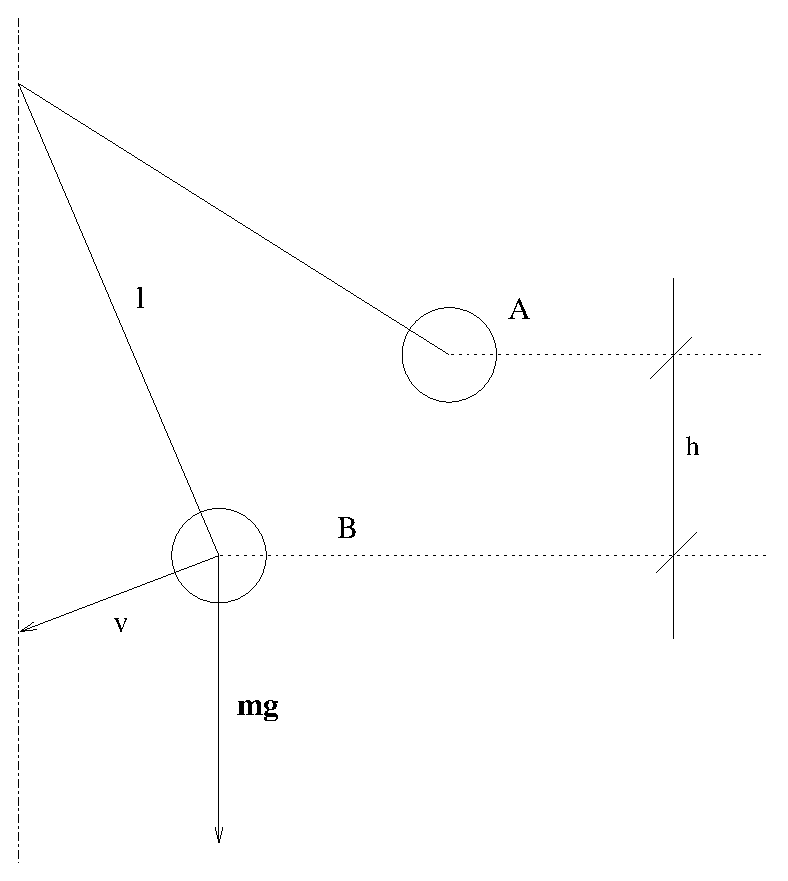
\includegraphics[scale=0.4]{immagini/fisica1/Pendolo_energia}
\end{figure}
Angoli non piccoli, $\ve T\bot \ve v \qquad \ve T\bot \ud\ve s$
\[\delta L=\ve T \cdotp \ud\ve s=0\]
\[U=mgh \qquad K=\frac{1}{2}mv^2\]
\[mgh+\frac{1}{2}mv^2=E=\const\]
A $\theta_0$ si trova nella posizione $A\quad K_A=0$
\[E_A=0+mgh\]
In $B$ $K_B\neq 0\quad E_B=K+mgh_B$
\[h=l-l\cos\theta\]
\[E_A=mg\left(l-l\cos\theta_0\right)\]
\[E_B=\frac{1}{2}mv^2+mg\left(l-l\cos\theta\right)\]
\[E_A=E_B\]
\[mgl\left(1-\cos\theta_0\right)=\frac{1}{2}mv^2+mgl\left(1-\cos\theta\right)\]
\[v^2=2gl(\cos\theta-\cos\theta_0)\]

\begin{Es}[arriva in alto?]
  \begin{figure}[htbp]
    \centering
    \includegraphics[scale=0.4]{immagini/fisica1/arriva_in_alto}
  \end{figure}
  La $\ve N$ non compie lavoro perché $\ve N\bot \ud\ve s$
  \[E_A=\frac{1}{2}mv_0^2 \qquad E_B=\frac{1}{2}mv_B^2+mg2R\]
  \[E_A=E_B \quad E_A=\frac{1}{2}mv_0^2=\frac{1}{2}mv_B^2+mg2R\]
  \[v_0^2=v_B^2+4gR\]
  Quando è in B
  \[mg+N=m\frac{v_B^2}{R}\qquad N=m\frac{v_B^2}{R}-mg\quad \text{per non cadere:}\quad N\geq0\]
  \[m\frac{v_B^2}{R}\geq mg\qquad v_B^2\geq gR\]
  \[v_{B\text{min}}^2=gR\qquad v_{0\text{min}}^2=gR+4gR\qquad v_{0\text{min}}=\sqrt{5gR}\]
\end{Es}